
\pagenumbering{arabic}

\chapter[Introdução e Justificativa]{Introdução e Justificativa}

Desde a invenção dos primeiros computadores em 1950, já existia uma certa discussão sobre o potencial de sua aplicação em áreas como a Medicina e a Biologia. Em 1968, A. A. Robertson  publicou um artigo com o título ``\textit{The use of computers in medicine with particular reference to general practice}'', porém, uma definição mais concreta sobre esta nova área da ciência que estava surgindo só começou a ser formulada em 1980 quando Edward Shortlife, Larry Fagan e Gio Wiederhold começaram a escrever o primeiro livro sobre Informática Médica para um curso de Medicina na Universidade de Stanford \cite{biomed_info}.

\section{Informática Biomédica}

De acordo com a terceira versão do livro ``\textit{Biomedical Informatics}'' publicada em 2006 por Shortlife, essa área de conhecimento corresponde ao estudo da informação biomédica, conectando dados e conhecimento, sendo responsável pelo armazenamento e recuperação dos dados, e da utilização de computadores para a solução de problemas médicos e auxílio na tomada de decisão.

Inicialmente esta área foi chamada de Informática Médica, sendo que o termo Informática Biomédica só começou a surgir a partir dos anos 90, com a expansão do Projeto Genoma Humano e da investigação e análise de dados aplicados em Biologia, através da conscientização de que os métodos e processos utilizados também poderiam ser aplicados na Biomedicina de uma maneira mais ampla e geral \cite{Kulikowski2012}.

Apesar de Informática Biomédica ser o termo mais adotado atualmente, ainda existe uma grande discussão sobre a real definição do seu significado e quais são as suas áreas de atuação. Um exemplo dessa discussão é o fato de que as associações representantes da área nos Estados Unidos ainda são chamadas de ``informática médica'' como a ``\textit{American Medical Informatics Association}'' e ``\textit{International Medical Informatics Association}''. No Brasil a associação representante desta área chama-se Sociedade Brasileira de Informática em Saúde (SBIS) \footnote{\url{http://www.sbis.org.br/}}, essa associação foi fundadada em 1986 pelo Prof. Renato Sabbatini com o objetivo de promover a troca de idéias e a apresentação de resultados nas área de Informática em Saúde, Telemedicina e Bioinformática.

De acordo com Bernstam \cite{Bernstam2010} em seu artigo ``\textit{What is Biomedical Informatics}'' publicado em 2010, a Informática Biomédica pode ser definida como a aplicação da Ciência da Informação e da Computação como dados e conhecimento para solução de problemas de interesse biomédicos.

\section{Bioinformática}

A Bioinformática é uma área multidisciplinar que integra os conhecimentos de diversas áreas diferentes como por exemplo: Biologia, Computação, Estatística, Matemática e Engenharia para realizar a análise de dados biológicos, além de construir ferramentas que permitam o armazenamento, organização, visualização e interpretação dos dados através do uso de um computador para realizar essas tarefas e gerar novo conhecimento.

A palavra Bioinformática foi utilizada pela primeira vez em um artigo publicado por Paulien Hogeweg em 1978 para descrever o estudo da informação em sistemas bióticos \cite{Hogeweg2011}. Desde então este termo se tornou mais abrangente, ganhando popularidade entre 1990 e 2000 no período chamado de revolução genômica quando passou a ser utilizado para representar a construção, manutenção e interpretação de grandes bancos de dados biológicos impulsionados pelo sucesso do Projeto Genoma Humano e o aumento da quantidade de dados biológicos disponíveis.

Apesar de Informática Biomédica e da Bioinformática serem áreas distintas, a pergunta que sempre surge neste ponto é qual seria então a interseção entre as duas áreas e esse assunto já foi amplamente discutido em estudos anteriores \cite{Practice2003, Martin-Sanchez2004}. De maneira geral podemos dizer que a Bioinformática possui um foco maior na Biologia Molecular enquanto a Informática Biomédica possui um foco maior na área Médica.

A associação que representa a área de Bioinformática no Brasil chama-se Associação Brasileira de Bioinformática e Biologia Computacional (AB3C) \footnote{\url{http://ab3c.cebio.org/}}.

\section{O Exoma}

Um éxon pode ser descrito como a parte do gene que fará parte do RNA maduro depois da remoção de todos os íntrons durante um processo de edição do RNA mensageiro que é chamado de \textit{RNA splicing}. A figura~\ref{fig:exon_image} apresenta o modelo de uma estrutura gênica com as suas regiões de íntrons, éxons e UTRs (\textit{Unstranslated Regions}) delimitadas com as cores vermelho, azul e cinza respectivamente.

\afterpage{
\begin{landscape}
\begin{figure}[p]
  \centering
    \Large\textbf{A estrutura de um Gene}\par\medskip
    \fbox{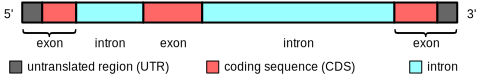
\includegraphics[width=1.4\textwidth]{../Figures/Gene_structure.png}}
    \caption[A estrutura de um Gene]{Esta figura mostra a estrutura simplificada de um gene com suas regiões de íntrons, éxons e UTRs (regiões não traduzidas). Fonte: \url{http://en.wikipedia.org/wiki/Exon}}
  \label{fig:exon_image} 
\end{figure}
\end{landscape}

\clearpage
}

Um exoma pode ser definido como a coleção de todos os éxons de um genoma. Essas  regiões correspondem a cerca de ~1.5\% do genoma humano (~30 Megabases) e estão divididas entre ~180,000 éxons. Apesar de constituir uma parte pequena do genoma, acredita-se que esta região contenha cerca de ~85\% das mutações associadas a doenças genéticas humanas \cite{Choi2009}. Isso demonstra a importância do estudo e da compreensão dessa região para ajudar na compreensão de doenças genéticas. Até fevereiro de 2015, 2937 genes associados a 4163 doenças mendelianas foram descobertos, porém cerca de 50\% das doenças mendelianas ainda não possuem um gene identificado. Portanto essa área ainda fornece grandes oportunidades para a descoberta de novos genes associados a doenças mendelianas \cite{Chong2015}. 


\section{Doenças Mendelianas}

Doenças Mendelianas são doenças genéticas que podem ser causadas por uma única mutação em um único gene. Além disso elas podem ser herdadas dos pais, ou seja, podem ser transmitidas de uma geração para outra de acordo com o modelo de herança proposto pelas leis de Mendel. Podemos citar como exemplos de doenças Mendelianas a anemia falciforme (OMIM:603903), a fibrose cística (OMIM:219700), a síndrome de Marfan (OMIM:154700) e a doença de Huntington (OMIM:143100). Existem atualmente mais de 4 mil doenças Mendelianas conhecidas de acordo com o site OMIM.

\section{Análise de Exomas para o diagnóstico de doenças Mendelianas}

Em 2008 \cite{Ng2008} publicaram um artigo contendo o sequenciamento do primeiro exoma humano (do pesquisador J. Craig Venter), mas apenas em 2009, foi publicado o primeiro artigo que utilizou o sequenciamento de exomas e o método de filtragem de variantes como uma prova de conceito para realizar a identificação do gene \textit{MYH3} (Gene ID: 4621) como sendo associado a Síndrome de Freeman-Sheldon (OMIM:193700) \cite{Ng2009}. Para identificar este gene foi necessário realizar o sequenciamento de 12 exomas, sendo 4 dos indivíduos afetados pela doença não relacionados e 8 indivíduos normais do projeto HapMap que foram utilizados como controles no processo de filtragem de variantes. Desde então centenas de outros estudos foram publicados com a utilização do sequenciamento de exomas de pacientes para descoberta de novas associações entre genes e doenças Mendelianas que até então ainda eram desconhecidas \cite{Bamshad2011a}.

A síndrome de Freeman-Sheldon (FSS) é uma doença genética causada por herança autossômica dominante, a forma mais conhecida pela literatura, e também por herança autossômica recessiva, ambas as formas são responsáveis por causar alterações ósseas e contraturas articulares levando a um fenótipo do paciente que é bastante característico.

A figura~\ref{fig:exome_filtering_example} mostra como foi o processo de filtragem de variantes que foi utilizado para a identificação do gene \textit{MYH3}. Podemos observar através desta figura que ao filtrar apenas por genes com mutações não sinônimas que estivessem presentes nos quatro indivíduos foi possível reduzir o número de genes candidatos para 2479 genes, ao eliminarem as mutações que estavam presentes apenas na última versão do dbSNP conseguiram diminuir a lista de genes candidatos para 53, ao utilizarem os dados dos 8 exomas controles do projeto HapMap conseguiram reduzir a lista de genes para 21, e por fim ao removerem os dados do dbSNP e do HapMap ao mesmo tempo, conseguiram reduzir a lista de genes candidatos para apenas 1 único gene. É importante notar que este gene também poderia ter sido encontrado utilizando outros critérios de filtragem como por exemplo o escore de SIFT e Polyphen-2 de cada variante. Este estudo mostrou que com a utilização de apenas 4 indivíduos não relacionados seria possível identificar o gene causador da doença Mendeliana investigada.

\afterpage{
\begin{landscape}
\begin{figure}[p]
  \centering
    \Large\textbf{Processo de Filtragem de Variantes para identificação de uma doença Mendeliana}\par\medskip
    \fbox{\includegraphics[width=1.4\textwidth]{../Figures/fss_filtering_process.png}}
    \caption[Processo de Filtragem de Variantes para identificação de uma doença Mendeliana]{Nesta imagem podemos verificar todas as etapas de filtragem que foram utilizadas para identificação do gene \textit{MYH3} como causador da síndrome de Freeman-Sheldon. Fonte: \cite{Ng2009}}
    
  \label{fig:exome_filtering_example}
\end{figure}
\end{landscape}

\clearpage
}

O gene \textit{MYH3} já era conhecido como sendo o causador síndrome de Freeman-Sheldon porém o estudo serviu como uma prova de conceito de que a tecnologia e o método poderiam ser utilizados para investigação de outras doenças onde o gene responsável ainda fosse desconhecido.

Ainda em 2009, Ng e o seu grupo \cite{Ng2010} descobriram a associação de um novo gene chamado \textit{DHODH} (Gene ID: 1723) como sendo o causador da Síndrome de Miller (OMIM\%263750) utilizando o mesmo método que havia sido validado pelo estudo anterior. Esta foi a primeira vez que a análise de exomas foi utilizada para identificação de um novo gene responsável por causar uma doença Mendeliana onde até então sua causa ainda era desconhecida.

Um estudo publicado em Fevereiro de 2015 \cite{Hu2015} realizou o sequenciamento do cromossomo X de 405 famílias com casos clínicos que ainda não haviam sido solucionados por outros métodos, e como resultado deste estudo, eles conseguiram identificar 7 novos genes associados a deficiência intelectual.

A figura~\ref{fig:exome_pubmed} mostra o crescimento do número de artigos publicados com a palavra ``\textit{exome}'' em títulos ou abstracts desde o ano de 2008 de acordo com o site Pubmed. 

Podemos observar que a partir de 2008 este número tem crescido a cada ano e que a previsão do número de artigos publicados em 2015 será ainda maior do que foi em 2014.

\afterpage{
\begin{landscape}

\begin{figure}[p]
    \centering
    \Large\textbf{Crescimento do número de artigos publicados com a palavra exome no Pubmed}\par\medskip
    \fbox{\includegraphics[width=1.5\textwidth]{../Figures/exome_pubmed.png}}
    \caption[Crescimento do número de artigos publicados com a palavra exome no Pubmed]{Nesta imagem podemos verificar o crescimento do número de artigos publicados com a palavra ``exome'' de acordo com o Pubmed ao longo dos últimos anos.}
    
  \label{fig:exome_pubmed}
\end{figure}
\end{landscape}

\clearpage
}

Esta técnica vem crescendo e se expandindo ao longo dos últimos anos e ainda deverá ser muito utilizada para realizar a investigação e o diagnóstico de doenças genéticas humanas. Apesar do sucesso comprovado deste método, ainda existem grandes desafios para que esta técnica seja completamente adotada e integrada dentro da prática clínica.

Atualmente existem poucas ferramentas desenvolvidas com o objetivo de auxiliar médicos e pesquisadores a analisarem este tipo de dado, e grande parte das ferramentas que existem, ainda exigem a execução de scripts e comandos manuais geralmente em um terminal Linux com o uso de parâmetros que possibilitem a exploração dos dados e a filtragem de variantes. A ausência de uma interface simples e amigável dificulta o acesso aos métodos e as informações por pessoas que não possuem conhecimentos sobre programação ou computadores.

Para este método atingir sua plenitude é preciso que existam programas práticos e acessíveis, que possibilitem a exploração dos dados não apenas por cientistas, mas também por médicos o outros profissionais da área da Saúde. 

É neste sentido que este trabalho foi iniciado, para ajudar traduzir os resultados obtidos a partir do sequenciamento de exomas e para tentar extrair informação útil deste tipo de dado para auxiliar no diagnóstico clínico de doenças Mendelianas.

\section{SNPs e Indels}

O Polimorfismo de Nucleotídeo Único (SNP) é uma variação genética causada pela alteração em um único par de base em uma posição específica do DNA.

A figura~\ref{fig:snp} mostra a representação gráfica de uma SNP e nela podemos observar a alteração de uma posição contendo GC para AT.

Os SNPs presentes nas regiões exônicas podem ser classificadas como sinônimas, ou seja, aquelas que não causam alteração na sequência de aminoácidos da proteína, e não-sinônimas, que são aquelas que causam alteração na sequência de aminoácidos da proteína. As mutações não-sinônimas podem ser classificadas como \textit{missense} e \textit{nonsense}. As mutações \textit{missense} são aquelas que causam uma substituição de um aminoácido por outro, e as mutações \textit{nonsense} são aquelas que causam a substituição de um aminoácido por um \textit{stop} códon, o que pode causar a produção de uma proteína não funcional.

\afterpage{
\begin{landscape}
\begin{figure}[p]
    \centering
    \Large\textbf{Representação gráfica de uma SNP}\par\medskip
    \fbox{\includegraphics[width=0.6\textwidth]{../Figures/Dna-SNP.png}}
    \caption[Representação gráfica de uma SNP]{Representação gráfica de uma SNP mostrando uma alteração de G->C para A->T. Fonte: \url{http://en.wikipedia.org/wiki/Single-nucleotide_polymorphism}}
  \label{fig:snp}  
\end{figure}
\end{landscape}

\clearpage
}

Indel é um polimorfismo que corresponde a adição ou remoção de uma pequena sequência de bases de DNA, sendo que a maioria ocorre em regiões de repetição em tandem.

Na figura~\ref{fig:indel} é apresentado a representação gráfica de uma indel. Podemos observar uma deleção de duas bases AC na parte de cima e da inserção de duas bases AC na parte de baixo. Existem muitas indels associadas a doenças humanos e este é um assunto já bastante discutido em estudos anteriores \cite{Taylor2004, Haraksingh2013}.

\afterpage{
\begin{landscape}

 \begin{figure}[p]
   \centering
      \Large\textbf{Representação gráfica de uma Indel}\par\medskip
      
      \fbox{\includegraphics[width=1\textwidth]{../Figures/indel.png}}
      
      \caption[Representação gráfica de uma Indel]{Podemos observar uma deleção de duas bases AC na parte de cima e da inserção de duas bases AC na parte de baixo. Fonte: \url{http://genome.sph.umich.edu/wiki/Indel}}
      
     \label{fig:indel}
 \end{figure}
\end{landscape}

\clearpage
}


\section{Projeto Genoma Humano}

O Projeto Genoma Humano \cite{Lander2001} foi um consórcio científico internacional coordenado pelo \textit{National Institutes of Health} (NIH) com o objetivo de mapear todos os genes humanos e realizar o sequenciamento dos 3 bilhões de nucleotídeos do genoma humano.  Esse projeto teve um custo aproximado de 3 bilhões de dólares e em 2001, 10 anos após o seu início do projeto, foi publicado o primeiro rascunho do genoma humano.

Em 1998 o pesquisador J. Craig Venter deu início a um projeto paralelo em sua empresa \textit{Celera Genomics} para sequenciar o genoma humano usando uma técnica conhecida por \textit{Shotgun Sequencing} \cite{Venter2001}. Esta técnica permitiu o sequenciamento do genoma humano através da quebra do DNA em pequenos fragmentos de tamanho entre 100 e 1000 pares de base de maneira que a montagem do genoma pudesse ser realizada através do uso de programas de computador. Para isso foi necessário atingir uma cobertura mínima de 12X, ou seja, cada base do genoma foi sequenciada pelo menos 12 vezes para que essa montagem fosse possível.

Ambos os projetos foram publicados em 2001 pelas revistas \textit{Nature} e \textit{Science} \cite{Lander2001, Venter2001}.


\section{Projeto 1000 Genomas}

O ``\textit{1000 Genomes Project}'' \cite{Abecasis2010, Abecasis2012} é um projeto de colaboração internacional criado em 2009 com o objetivo de produzir um catálogo abrangente sobre as variações genéticas humanas. Até o momento já foram sequenciados e genotipados 2504 indivíduos\footnote{\url{http://www.1000genomes.org/data}}, esses dados estão disponibilizados de forma totalmente pública na internet para qualquer pesquisador que tiver interesse em realizar o download para analisá-los. Isso passou a permitir o uso desses dados de forma a auxiliar a clínica médica para realizar análises de exomas de pacientes e por exemplo para fazer a comparação de grupos de indivíduos normais presentes nesses bancos de dados com pacientes clínicos permitindo a eliminação de variantes controles que estivessem presentes no grupo de indivíduos de uma população.

Na tabela~\ref{1000genomes_ancestry} apresentamos informações sobre o número dos indivíduos que foram sequenciados e os grupos de ancestralidade que foram definidos pelos pesquisadores do projeto \textit{1000 Genomes}.

Site: \url{http://www.1000genomes.org}

\afterpage{
\begin{landscape}
\begin{table}[p]
\centering
\caption[Informações sobre a ancestralidade dos indivíduos que foram sequenciados pelo projeto \textit{1000 Genomes}]{Informações sobre a ancestralidade dos indivíduos que foram sequenciados pelo projeto \textit{1000 Genomes}.
Fonte: \url{http://www.1000genomes.org/about} }
\scalebox{1.5}{
\begin{tabular}{|l|l|}
\hline
\textbf{Populações}                       & \textbf{Número final de amostras} \\ \hline
\textbf{Ancestralidade Leste-Asiática}  & 504                           \\ \hline
\textbf{Ancestralidade Sul-Asiática} & 489                           \\ \hline
\textbf{Ancestralidade Africana}     & 661                           \\ \hline
\textbf{Ancestralidade Européria}    & 503                           \\ \hline
\textbf{Ancestralidade Ameríndia}    & 347                           \\ \hline
\textbf{Total}                            & \textbf{2504}                \\ \hline
\end{tabular}
}
\label{1000genomes_ancestry}
\end{table}
\end{landscape}

\clearpage
}


\afterpage{
\begin{landscape}

\begin{figure}[p]
  \centering
    \Large\textbf{Medicina Personalizada}\par\medskip
    \fbox{\includegraphics[width=0.9\textwidth]{../Figures/Personalized_medicine.png}}
    \caption[Medicina Personalizada]{Aqui podemos verificar que Medicina Personalizada é um termo que relaciona a Medicina Tradicional, a Genômica Personalizada e a Farmacogenômica. Fonte: \cite{Fernald2011a}}
  \label{fig:personalized_medicine}  
\end{figure}
\end{landscape}

\clearpage
}

\section{Projeto de Sequenciamento do Exoma}

O \textit{Exome Sequencing Project} (ESP) \cite{Fu2013} realizou até o momento o sequenciamento de 6515 exomas e embora os genótipos dos indivíduos não estejam disponíveis para download, é possível obter informações sobre a frequência das variantes que foram encontradas e este valor pode ser utilizado no processo de filtragem de variantes de indivíduos que possuam uma Doença Mendeliana específica.

Site: \url{http://evs.gs.washington.edu/EVS}

\section{Medicina Personalizada / Medicina de Precisão}

O termo ``Medicina Personalizada'' começou a surgir a partir de 1999 quando Robert Langreth e Michael Waldholz publicaram no jornal ``\textit{The Oncologist}'' o primeiro artigo com uma definição mais próxima da que temos atualmente sobre essa nova área da medicina \cite{Langreth1999}. A Medicina Personalizada é um modelo de saúde que propõe a realização de práticas utilizando dados como o perfil genômico do paciente para a tomada de decisão médica, com o objetivo de direcionar o melhor tratamento específico para cada paciente de acordo essas informações.

Na figura~\ref{fig:personalized_medicine} apresentamos uma imagem com a relação entre a Medicina Tradicional, a Genômica Personalizada e a Farmacogenômica. Essa área atualmente tem sido chamada de Medicina de Precisão \cite{Collins2015, Jameson} por ser um termo que representa melhor a aplicação dos dados genômicos de uma forma direcionada para atender as necessidades clínicas de cada paciente.


